%==========================================
%
% SIBGRAPI 2026 paper template
% Example of IEEEtran.cls
%
%==========================================

% *** Authors should verify (and, if needed, correct) their LaTeX system  ***
% *** with the testflow diagnostic prior to trusting their LaTeX platform ***
% *** with production work. The IEEE's font choices and paper sizes can   ***
% *** trigger bugs that do not appear when using other class files.       ***                          ***
% The testflow support page is at:
% http://www.michaelshell.org/tex/testflow/

\documentclass[10pt,conference]{IEEEtran}
\renewcommand{\arraystretch}{0.92}

% Some very useful LaTeX packages include:
% (uncomment the ones you want to load)



% *** MISC UTILITY PACKAGES ***
%
%\usepackage{ifpdf}
% Heiko Oberdiek's ifpdf.sty is very useful if you need conditional
% compilation based on whether the output is pdf or dvi.
% usage:
% \ifpdf
%   % pdf code
% \else
%   % dvi code
% \fi
% The latest version of ifpdf.sty can be obtained from:
% http://www.ctan.org/pkg/ifpdf
% Also, note that IEEEtran.cls V1.7 and later provides a builtin
% \ifCLASSINFOpdf conditional that works the same way.
% When switching from latex to pdflatex and vice-versa, the compiler may
% have to be run twice to clear warning/error messages.

\usepackage{xcolor}
\usepackage{tikz}
\usepackage{fontawesome5}
\usepackage{float}
\usepackage{booktabs}
\usepackage{multirow}
\usepackage{amssymb}
\usetikzlibrary{positioning, fit, arrows.meta, backgrounds}

% *** CITATION PACKAGES ***
%
\usepackage{cite}
% cite.sty was written by Donald Arseneau
% V1.6 and later of IEEEtran pre-defines the format of the cite.sty package
% \cite{} output to follow that of the IEEE. Loading the cite package will
% result in citation numbers being automatically sorted and properly
% "compressed/ranged". e.g., [1], [9], [2], [7], [5], [6] without using
% cite.sty will become [1], [2], [5]--[7], [9] using cite.sty. cite.sty's
% \cite will automatically add leading space, if needed. Use cite.sty's
% noadjust option (cite.sty V3.8 and later) if you want to turn this off
% such as if a citation ever needs to be enclosed in parenthesis.
% cite.sty is already installed on most LaTeX systems. Be sure and use
% version 5.0 (2009-03-20) and later if using hyperref.sty.
% The latest version can be obtained at:
% http://www.ctan.org/pkg/cite
% The documentation is contained in the cite.sty file itself.


% *** GRAPHICS RELATED PACKAGES ***
%
\ifCLASSINFOpdf
   \usepackage{graphicx}
  % declare the path(s) where your graphic files are
   \graphicspath{{img/}}
  % and their extensions so you won't have to specify these with
  % every instance of \includegraphics
   \DeclareGraphicsExtensions{.pdf,.jpeg,.png}
\else
  % or other class option (dvipsone, dvipdf, if not using dvips). graphicx
  % will default to the driver specified in the system graphics.cfg if no
  % driver is specified.
   \usepackage[dvips]{graphicx}
  % declare the path(s) where your graphic files are
   \graphicspath{{../img/}}
  % and their extensions so you won't have to specify these with
  % every instance of \includegraphics
   \DeclareGraphicsExtensions{.eps}
\fi

% *** MATH PACKAGES ***
%
\usepackage[cmex10]{amsmath}
% A popular package from the American Mathematical Society that provides
% many useful and powerful commands for dealing with mathematics.
%
% Note that the amsmath package sets \interdisplaylinepenalty to 10000
% thus preventing page breaks from occurring within multiline equations. Use:
\interdisplaylinepenalty=2500
% after loading amsmath to restore such page breaks as IEEEtran.cls normally
% does. amsmath.sty is already installed on most LaTeX systems. The latest
% version and documentation can be obtained at:
% http://www.ctan.org/pkg/amsmath
\usepackage{amsthm}
\newtheorem{definition}{Definition}

% *** SPECIALIZED LIST PACKAGES ***
%
\usepackage{algorithm}
\usepackage{algorithmic}

% *** ALIGNMENT PACKAGES ***
%
\usepackage{array}
% *** SUBFIGURE PACKAGES ***
\ifCLASSOPTIONcompsoc
  \usepackage[caption=false,font=normalsize,labelfont=sf,textfont=sf]{subfig}
\else
  \usepackage[caption=false,font=footnotesize]{subfig}
\fi

\usepackage{stfloats}

% *** PDF, URL AND HYPERLINK PACKAGES ***
%
\usepackage{url}


% correct bad hyphenation here
\hyphenation{op-tical net-works semi-conduc-tor}

%------------------------------------------------------------------------- 
% change the % on next lines to produce the final camera-ready version 
\newif\iffinal
%\finalfalse
\finaltrue
\newcommand{\cmtid}{99999}
%------------------------------------------------------------------------- 

\iffinal
\else
\usepackage[switch]{lineno}
\fi

\begin{document}
\bstctlcite{IEEEexample:BSTcontrol}
\title{NeRF Architectures under Sparse-View Conditions: A Systematic Benchmarking Methodology}

% author names and affiliations
% use a multiple column layout for up to two different
% affiliations for over three affiliations, or if they all won't fit within the width
% of the page, use this alternative format: 
\author{\IEEEauthorblockN{
Felipe G. Silva\IEEEauthorrefmark{1},
Leandro A. Neves\IEEEauthorrefmark{1},
Guilherme F. Roberto\IEEEauthorrefmark{1},
Thiago Pozati\IEEEauthorrefmark{1},
Domingos Oliveira\IEEEauthorrefmark{2}\textsuperscript{,}\IEEEauthorrefmark{3}, \\
Adriano B. Silva\IEEEauthorrefmark{3},
Tha\'ina A. A. Tosta\IEEEauthorrefmark{4} and
Marcelo Z. do Nascimento\IEEEauthorrefmark{3}
}

\IEEEauthorblockA{\IEEEauthorrefmark{1}Department of Computer Science and Statistics (DCCE).  São Paulo State University (UNESP),\\ São José do Rio Preto, SP, Brazil. Email: felipe.gomes-silva@unesp.br}

\IEEEauthorblockA{\IEEEauthorrefmark{2}Federal Institute of Education, Science and Technology of São Paulo (IFSP), São Paulo, SP, Brazil.}

\IEEEauthorblockA{\IEEEauthorrefmark{3}Faculty of Computer Science (FACOM), Federal University of Uberlândia (UFU), Uberlândia, MG, Brazil}

\IEEEauthorblockA{\IEEEauthorrefmark{4}Department of Computing and Mathematics, University of São Paulo (USP), Ribeirão Preto, SP, Brazil}
}

% make the title area
\maketitle

\begin{abstract}
Novel view synthesis from few input images ($N \le 10$) involves a direct trade-off between learned geometric priors, optimization stability, and rendering speed. This work presents a reproducible benchmarking methodology that compares generalizable implicit architectures (PixelNeRF and GNT) under five fine-tuning strategies (Full Fine-Tuning, PFT-Decoder, PFT-Backbone, BitFit, and PEFT-LoRA) against implicit and explicit per-scene representations (Instant-NGP, Nerfacto, and 3D Gaussian Splatting via Splatfacto) on the LLFF benchmark. Quantitative and qualitative evaluations were conducted using PSNR, SSIM, LPIPS, training time, rendering throughput (FPS), and dynamic VRAM consumption. Per-scene optimization achieved the highest performance under 10 input views: Nerfacto reached 27.11 dB PSNR, 0.875 SSIM, and 0.171 LPIPS, while Splatfacto rendered novel views at 200.7 FPS using 0.10 GB of VRAM (24.80 dB PSNR). Under three input views ($N=3$), modular parameter adaptation prevented representational collapse in pre-trained models: GNT adapted with PFT-Decoder (15.07 dB) and PEFT-LoRA ($r=4$, 14.57 dB) matched Full Fine-Tuning accuracy while reducing adaptation time by 16.3\% ($\sim$5 min) and outperforming Instant-NGP (14.06 dB), although limited by volumetric ray-marching latency ($\le 0.015$ FPS). The custom Nerfstudio wrappers and benchmarking scripts were publicly released to support reproducible and continuous evaluation.
\end{abstract}

% For peerreview papers, this IEEEtran command inserts a page break and
% creates the second title. It will be ignored for other modes.
\IEEEpeerreviewmaketitle

\section{Introduction}
\label{sec:intro}

Neural Radiance Fields (NeRFs) and explicit point-based representations such as 3D Gaussian Splatting (3DGS) have become standard approaches for novel view synthesis \cite{mildenhall2020nerfrepresentingscenesneural, kerbl3Dgaussians, Tancik2023}. However, most neural rendering methods require dense multi-view supervision and long optimization times, which limits their application in acquisition-constrained settings such as mobile scanning, robotic navigation, and 3D biomedical imaging \cite{ijms24076747, niemeyer2022regnerf}.

Recent architectures have addressed these limitations through two distinct approaches. Per-scene methods reduce training and inference costs using multiresolution hash grids, as in Instant-NGP \cite{muller2022} and Nerfacto \cite{Tancik2023}, or explicit tile-based Gaussian rasterization, as in Splatfacto \cite{kerbl3Dgaussians}. In parallel, generalizable architectures learn multi-view priors across large datasets to synthesize novel views from few source images, as demonstrated by PixelNeRF \cite{yu2021pixelnerfneuralradiancefields} and the Generalizable NeRF Transformer (GNT) \cite{t2023attentionnerfneeds}. Although generalizable models support feed-forward inference and short fine-tuning, their behavior under parameter-efficient fine-tuning (PEFT) and their computational trade-offs relative to implicit and explicit per-scene baselines have largely been evaluated under separate experimental protocols \cite{kulhanek2025nerfbaselinesconsistentreproducibleevaluation}.

This work proposes a standardized benchmarking methodology to evaluate generalizable and per-scene neural rendering architectures under sparse-view conditions ($N \le 10$ on the LLFF dataset). Reconstruction fidelity (PSNR, SSIM \cite{wang2004image}, and LPIPS \cite{zhang2018unreasonable}) and computational performance (training time, rendering throughput in FPS, and peak dynamic VRAM) were jointly measured. The main contributions of this study are:
\begin{itemize}\setlength{\itemsep}{1pt}\setlength{\parskip}{0pt}
\item A unified evaluation protocol comparing per-scene models (Instant-NGP, Nerfacto, and Splatfacto/3DGS) and pre-trained generalizable models (PixelNeRF and GNT) across zero-shot and stratified $K$-fold fine-tuning regimes.
\item Publicly released Nerfstudio integration wrappers (\texttt{nerfstudio-gnt} and \texttt{nerfstudio-pixelnerf}) implementing five adaptation strategies (Full-FT, PFT-Decoder, PFT-Backbone, BitFit, and PEFT-LoRA) with in-place weight merging for inference.
\end{itemize}

\section{Theoretical Background}
\label{sec:fund}

\subsection{Neural Radiance Fields and Volumetric Rendering}
Neural Radiance Fields (NeRFs) model continuous three-dimensional scene geometry and view-dependent appearance by mapping spatial coordinates and viewing directions to volumetric density and emitted radiance using Multilayer Perceptrons (MLPs) \cite{mildenhall2020nerfrepresentingscenesneural}. Given a spatial position $\mathbf{x} = (x, y, z)$ and a unit viewing direction $\mathbf{d} = (\theta, \phi)$, the network outputs differential volume density $\sigma(\mathbf{x}) \in \mathbb{R}_{\geq 0}$ and directional color $\mathbf{c} \in [0, 1]^3$:
\begin{equation}
\gamma(\mathbf{x}, \mathbf{d}) \rightarrow \mathbf{v}, \quad F_\theta'(\mathbf{v}) \rightarrow (\sigma, \mathbf{c})
\label{eq:nerf_formulation}
\end{equation}
where $\theta$ denotes the trainable network parameters, $F_\theta'$ represents the MLP, and $\gamma$ is a positional encoding mapping coordinates into a higher-dimensional space $\mathbf{v}$ through sinusoidal basis functions, enabling the network to represent high-frequency geometric and textural variations \cite{mildenhall2020nerfrepresentingscenesneural}.

Synthesizing the color observed by a camera pixel involves casting a ray $\mathbf{r}(t) = \mathbf{o} + t\mathbf{d}$ between near and far bounds $(t_n, t_f)$ and evaluating the volumetric rendering integral \cite{mildenhall2020nerfrepresentingscenesneural}:
\begin{equation}
\hat{C}(\mathbf{r}) = \int_{t_n}^{t_f} T(t) \sigma(\mathbf{r}(t)) \mathbf{c}(\mathbf{r}(t), \mathbf{d}) \, dt
\label{eq:vol_render}
\end{equation}
where $T(t) = \exp\left(-\int_{t_n}^t \sigma(\mathbf{r}(s)) \, ds\right)$ denotes the accumulated transmittance along the ray. Numerical approximation evaluates this continuous integral through stratified quadrature sampling, compositing discrete alpha-blended color samples along each sampled ray.

\subsection{Architectural Optimizations and Generalization}
Standard coordinate-based MLPs achieve remarkable visual fidelity, yet their dense parameter evaluations impose computational and convergence bottlenecks. Accelerating this optimization has motivated hybrid spatial representations that replace global positional encodings with explicit multiresolution data structures. Instant-NGP maps spatial coordinates to multiscale hash tables of trainable feature vectors, reducing convergence times from hours to seconds \cite{muller2022}. Nerfacto builds upon this paradigm by coupling multiresolution hash grids with proposal sampling, camera pose refinement, spherical harmonics, and appearance embeddings, achieving a balanced trade-off between rendering speed and perceptual quality \cite{Tancik2023}.

These per-scene representations, however, rely on dense multi-view coverage with substantial angular overlap. Practical applications, ranging from mobile capture and robotic navigation to biomedical imaging, such as 3D histology and holotomography, routinely face data acquisition constraints where only a few sparse views are available \cite{ijms24076747}. Under such sparse regimes, per-scene optimization becomes heavily underconstrained, possibly resulting in geometric degradation, false surfaces, and floating artifacts \cite{niemeyer2022regnerf, jain2021dietnerf}.

To overcome these data limitations, generalizable NeRFs learn inductive structural and multi-view priors across large scene collections, enabling feed-forward synthesis on novel target environments \cite{yu2021pixelnerfneuralradiancefields, chen2021mvsnerffastgeneralizableradiance, wang2021ibrnet, t2023attentionnerfneeds}. PixelNeRF projects query 3D points onto 2D image planes, extracting spatial feature vectors via a convolutional backbone (ResNet) to condition a coordinate-based radiance MLP \cite{yu2021pixelnerfneuralradiancefields}. Addressing the locality limits of convolutional operators, the Generalizable NeRF Transformer (GNT) replaces the CNN backbone with a Vision Transformer (ViT) and substitutes the terminal MLP with a cross-attention transformer, aggregating multi-view features directly along epipolar lines \cite{t2023attentionnerfneeds}.

\subsection{Fine-Tuning Strategies and Parameter-Efficient Regimes in NeRFs}
\label{sec:ft_theory}

Pre-trained generalizable models capture rich geometric and cross-view priors during large-scale pre-training \cite{yu2021pixelnerfneuralradiancefields, t2023attentionnerfneeds}. Deploying these networks directly in a zero-shot (ZS) regime on novel real-world scenes exposes them to pronounced domain shifts caused by discrepancies in sensor intrinsics, illumination conditions, and complex out-of-distribution textures \cite{mildenhall2019locallightfieldfusion, niemeyer2022regnerf}. In sparse-view settings ($N \le 10$), feed-forward zero-shot predictions frequently suffer from spatial ambiguities and lack high-frequency details, exhibiting noticeable isotropic blurring \cite{yu2021pixelnerfneuralradiancefields, chen2021mvsnerffastgeneralizableradiance}.

To bridge this domain gap, generalizable architectures employ fine-tuning (FT), optimizing network weights directly on the sparse target observations using the photometric reconstruction loss \cite{yu2021pixelnerfneuralradiancefields, chen2021mvsnerffastgeneralizableradiance}:
\begin{equation}
\mathcal{L}_{\text{photo}} = \frac{1}{|\mathcal{R}|} \sum_{\mathbf{r} \in \mathcal{R}} \|\hat{C}(\mathbf{r}) - C(\mathbf{r})\|_2^2
\label{eq:photo_loss}
\end{equation}
where $\mathcal{R}$ denotes a batch of synthesized rays and $C(\mathbf{r})$ represents the observed ground-truth pixel color.

Nevertheless, unconstrained gradient descent under view sparsity constitutes an ill-posed inverse problem \cite{jain2021dietnerf, niemeyer2022regnerf, roessle2022dense}. When high-capacity architectures are optimized against sparse camera rays without dense geometric constraints, the representation becomes susceptible to representational collapse \cite{jain2021dietnerf, niemeyer2022regnerf}. The network easily overfits to ray-specific photometric objectives by creating degenerate density floaters near camera centers, underperforming in global 3D consistency and degrading novel view synthesis quality \cite{niemeyer2022regnerf,roessle2022dense}.

This tension between model adaptation capacity and optimization stability parallels the challenges encountered in fine-tuning deep learning models across language, vision, and multimodal domains under scarce downstream supervision~\cite{hu2021lora, zaken2022bitfit, gupta2024beyondlora}. In their comprehensive benchmarking study of foundation model adaptation, Gupta et al. demonstrate that updating all model weights under limited target data destabilizes pre-trained representations, increases optimizer memory overhead, and can lead to overfitting. To address these vulnerabilities, the same authors formalize a comparative taxonomy comprising full model tuning, modular parameter freezing, selective parameter updates, and low-rank reparameterization. Transposing this modular methodology to generalizable neural rendering yields five distinct FT strategies~\cite{gupta2024beyondlora}:

\subsubsection{Full Fine-Tuning (Full-FT)}

All network parameters $\Theta = \{W, b\}$ across the feature extraction backbone and the volumetric rendering network are simultaneously updated via backpropagation. Although offering unconstrained representational capacity, Full-FT requires maintaining full optimizer moment tensors for every weight, incurring substantial memory overhead and heightening vulnerability to representational collapse when supervised by sparse views \cite{niemeyer2022regnerf,gupta2024beyondlora}.

\subsubsection{Partial Fine-Tuning: Decoder (PFT-Decoder)}
Gradient updates are restricted exclusively to the downstream volumetric rendering head—the cross-attention transformer in GNT \cite{t2023attentionnerfneeds} or the radiance MLP in PixelNeRF \cite{yu2021pixelnerfneuralradiancefields}—while the spatial feature extraction backbone remains frozen. Freezing the 2D perceptual layers preserves the generalizable representations established during pre-training, directing gradient updates solely toward refining multi-view radiance aggregation and scene-specific illumination \cite{gupta2024beyondlora}.

\subsubsection{Partial Fine-Tuning: Backbone (PFT-Backbone)}
Inverting the modular restriction, PFT-Backbone freezes the volumetric rendering head and updates solely the 2D feature extractor (the ResNet in PixelNeRF or the shallow patch embedder in GNT). This configuration enables the model to align its low-level perceptual feature maps with out-of-distribution textures and sensor profiles, leaving the pre-trained volumetric ray-marching logic undisturbed.

\subsubsection{Selective PEFT - BitFit}
BitFit isolates and optimizes exclusively the additive bias vectors $b \in \mathbb{R}^{d_{\text{out}}}$ of linear and convolutional transformations, keeping all projection weight matrices $W \in \mathbb{R}^{d_{\text{out}} \times d_{\text{in}}}$ strictly frozen \cite{zaken2022bitfit}:
\begin{equation}
y = W x + (b + \Delta b)
\label{eq:bitfit}
\end{equation}
As demonstrated in foundation model benchmarks by Ben Zaken et al. \cite{zaken2022bitfit} and Gupta et al. \cite{gupta2024beyondlora}, modifying solely the additive biases (typically representing less than $0.5\%$ of the total parameter count) acts as an effective structural regularizer. This parameter isolation stabilizes the optimization trajectory, preventing representational drift while providing sufficient flexibility to adjust activation thresholds for target scene alignment.

\subsubsection{Additive PEFT: Low-Rank Adaptation (PEFT-LoRA)}
LoRA freezes pre-trained weight matrices $W_0 \in \mathbb{R}^{d_{\text{out}} \times d_{\text{in}}}$ and parameterizes weight increments through a low-rank decomposition \cite{hu2021lora}:
\begin{equation}
W' = W_0 + \Delta W = W_0 + \frac{\alpha}{r} B A
\label{eq:lora}
\end{equation}
where $B \in \mathbb{R}^{d_{\text{out}} \times r}$ and $A \in \mathbb{R}^{r \times d_{\text{in}}}$ are low-rank factor matrices with rank $r \ll \min(d_{\text{in}}, d_{\text{out}})$, and $\alpha$ is a constant scaling hyperparameter. Matrix $A$ is initialized from a Gaussian distribution and $B$ is initialized to zero, ensuring $\Delta W = 0$ at the onset of adaptation. Restricting updates to an intrinsic low-dimensional subspace drastically curtails trainable parameters and optimizer memory during fine-tuning. Furthermore, as observed by Gupta et al. \cite{gupta2024beyondlora}, low-rank constraints act as an implicit regularizer that prevents catastrophic collapse when adapting deep foundational architectures to scarce downstream data.

Understanding the interaction between these modular fine-tuning strategies, generalizable priors, and per-scene representations requires a unified, reproducible benchmarking protocol, as formalized in the subsequent section.

\section{Materials and Methods}
\label{sec:methods}

This section describes the experimental methodology used to evaluate computational efficiency and reconstruction fidelity across neural rendering architectures under sparse-view conditions. Figure~\ref{fig:pipeline} illustrates the three stages of the pipeline: (i) dataset preparation and sparse-view sampling; (ii) model configuration across generalizable adaptation and per-scene training regimes; and (iii) quantitative and qualitative evaluation on held-out views.

\begin{figure}[!t]
\centering
\resizebox{0.9\linewidth}{!}{%
\begin{tikzpicture}[
  >=stealth,
  block/.style={
    rectangle, draw=black!30, thick, fill=white,
    minimum width=4.1cm, minimum height=0.95cm,
    text centered, rounded corners=3pt, font=\tiny,
    align=center
  },
  line/.style={draw, thick, black!45, ->, >=stealth, rounded corners=2pt}
]

% --- LEVEL 1 & 2: Dados Iniciais ---
\node[block] (data) at (0, 0) {
  \textbf{\faDatabase\ Dataset} \\[0.5mm] 
  LLFF ($8$ scenes, $504 \times 378$)
};

\node[block] (split) at (0, -1.45) {
  \textbf{\faProjectDiagram\ Split Generation} \\[0.5mm] 
  Uniform \& Random (seed 42, $N \in \{3, 6, 10\}$)
};
\draw[line] (data.south) -- (split.north);


% --- LEVEL 3: Bifurcação dos Modelos ---
\node[block] (gen_models) at (-2.3, -3.1) {
  \textbf{\faBrain\ Generalizable Models} \\[0.5mm] 
  PixelNeRF $\cdot$ GNT
};

\node[block] (ps_models) at (2.3, -3.1) {
  \textbf{\faCogs\ Per-Scene Models} \\[0.5mm] 
  Instant-NGP $\cdot$ Nerfacto $\cdot$ Splatfacto
};

% Setas do Split para os Modelos
\draw[line] (split.south) -- ++(0,-0.32) -| (gen_models.north);
\draw[line] (split.south) -- ++(0,-0.32) -| (ps_models.north);


% --- LEVEL 4: Regimes de Treino ---
\node[block] (gen_reg) at (-2.3, -4.55) {
  \textbf{\faTasks\ Regimes} \\[0.5mm] 
  Zero-Shot, Fine-Tuning ($500$ steps)
};

\node[block] (ps_reg) at (2.3, -4.55) {
  \textbf{\faTasks\ Regime} \\[0.5mm] 
  Per-Scene ($N=10$, $30\text{k}$ steps)
};

% Setas dos Modelos para os Regimes
\draw[line] (gen_models.south) -- (gen_reg.north);
\draw[line] (ps_models.south) -- (ps_reg.north);


% --- LEVEL 5 & 6: Avaliação e Métricas ---
\node[block] (eval) at (0, -6.2) {
  \textbf{\faVial\ Evaluation} \\[0.5mm] 
  Unified Protocol (\texttt{llffhold=8})
};

% Setas dos Regimes convergindo para Avaliação
\draw[line] (gen_reg.south) -- ++(0,-0.32) -| ([xshift=-2.5mm]eval.north);
\draw[line] (ps_reg.south) -- ++(0,-0.32) -| ([xshift=2.5mm]eval.north);

\node[block] (metrics) at (0, -7.65) {
  \textbf{\faChartBar\ Metrics} \\[0.5mm] 
  \textbf{Qual:} PSNR, SSIM, LPIPS \ $|$ \ \textbf{Perf:} Time, FPS, VRAM
};
\draw[line] (eval.south) -- (metrics.north);


% --- BACKGROUND (Ambiente Isolado) ---
\begin{scope}[on background layer]
  \node[draw=black!20, dashed, fill=black!2, rounded corners=5pt, 
        inner xsep=12pt, inner ysep=15pt, 
        fit=(data)(split)(gen_models)(ps_models)(gen_reg)(ps_reg)(eval)(metrics),
        label={[anchor=south east, font=\scriptsize\color{black!60}]south east:
        {\faDocker} Docker \ $|$ \ NVIDIA GTX 1660S \ $|$ \ CUDA 12.6}] (env) {};
\end{scope}

\end{tikzpicture}%
}
\caption{Proposed benchmarking pipeline. COLMAP-calibrated sparse splits ($N \in \{3, 6, 10\}$) were evaluated across two architectural branches inside an isolated Docker environment: generalizable models under Zero-Shot and five fine-tuning strategies, and per-scene baselines trained to convergence, assessed via visual fidelity (PSNR, SSIM, LPIPS) and computational metrics (Time, FPS, VRAM).}
\label{fig:pipeline}
\end{figure}


\subsection{Dataset \& Splits}
\label{sec:data}
All experiments were conducted on the Local Light Field Fusion (LLFF) dataset \cite{mildenhall2019locallightfieldfusion}, which contains 8 forward-facing real-world scenes with COLMAP-calibrated camera poses and depth bounds, downscaled by a factor of 8 ($504 \times 378$ pixels). Following the few-shot evaluation protocol of Niemeyer et al.\ \cite{niemeyer2022regnerf}, every 8th image (\texttt{llffhold=8}) was reserved for testing, while the training subsets were restricted to $N \in \{3, 6, 10\}$ views. Two view selection criteria were compared on the \textit{fern} scene ($N=10$, Table~\ref{tab:split}): (i) \textit{Uniform}, where training views were sampled by linear interpolation over the dataset indices along the camera trajectory; and (ii) \textit{Random}, where views were drawn using a fixed seed (\texttt{seed=42}). Uniform sampling yielded higher PSNR across all tested models (up to $+0.54$ dB on PixelNeRF and $+0.15$ dB on GNT) and was therefore adopted for all remaining experiments.

\begin{table}[!t]
\centering
\caption{Comparison between uniform and random training view selection under $N=10$ views on the \textit{fern} scene. Uniform sampling along the camera trajectory improved reconstruction metrics across both generalizable and per-scene models.}
\label{tab:split}
\scriptsize
\begin{tabular*}{\linewidth}{@{\extracolsep{\fill}}llcccc}
\toprule
Model & Split & PSNR $\uparrow$ & SSIM $\uparrow$ & LPIPS $\downarrow$ & $\Delta$PSNR \\
\midrule
\multirow{2}{*}{PixelNeRF}
  & Uniform   & 6.98   & 0.047    & 0.846    & \multirow{2}{*}{\textbf{+0.54}} \\
  & Random    & 6.44   & 0.042    & 0.840    &                        \\
\midrule
\multirow{2}{*}{GNT}
  & Uniform   & 10.34  & 0.179    & 0.738    & \multirow{2}{*}{+0.15} \\
  & Random    & 10.19  & 0.184    & 0.742    &                        \\
\midrule
\multirow{2}{*}{Instant-NGP}
  & Uniform   & \textbf{13.57} & \textbf{0.231} & \textbf{0.627} & \multirow{2}{*}{+0.06} \\
  & Random    & 13.51  & 0.229    & 0.630    &                        \\
\midrule
\multirow{2}{*}{Nerfacto}
  & Uniform   & 12.04  & 0.227    & 0.809    & \multirow{2}{*}{+0.11} \\
  & Random    & 11.93  & 0.226    & 0.865    &                        \\
\bottomrule
\end{tabular*}
\end{table}

Standardized execution parameters were applied across the benchmark. Camera pose refinement was disabled in Nerfacto because equivalent pose optimization is not natively supported by the other evaluated architectures. Mixed-precision training was enabled for all models, and the hash table capacity in Instant-NGP and Nerfacto was set to $2^{16}$ with white background compositing. For GNT, structural hyperparameters were kept at 48 coarse and fine samples per ray, a transformer depth of 8, and a feature width of 64 \cite{t2023attentionnerfneeds}.

\subsection{Models \& Training Regimes}
\label{sec:regimes}
Five representative architectures were evaluated across two modeling groups: generalizable implicit networks (PixelNeRF \cite{yu2021pixelnerfneuralradiancefields} and GNT \cite{t2023attentionnerfneeds}) and per-scene baselines comprising implicit hash grids (Instant-NGP \cite{muller2022} and Nerfacto \cite{Tancik2023}) and explicit 3D Gaussian primitives (Splatfacto \cite{kerbl3Dgaussians}). Three operational regimes were defined: (i) \textit{Zero-Shot (ZS)}, where pre-trained generalizable weights were evaluated directly without gradient updates; (ii) \textit{Fine-Tuning (FT)}, where pre-trained generalizable models were adapted on sparse target views; and (iii) \textit{Per-Scene}, where baseline representations were trained from scratch on $N=10$ views for $30,000$ iterations.

\subsubsection{Fine-Tuning Strategies and Implementation}
Custom Nerfstudio wrapper packages (\texttt{nerfstudio-gnt} and \texttt{nerfstudio-pixelnerf}\footnote{Repositories and packages: \url{https://github.com/Felipe-gsilva/Few-Shot-NeRFs/} and \url{https://github.com/Felipe-gsilva/nerf-ann-paper/}.}) were implemented with a shared adaptation module (\texttt{adaptation.py}) to execute the five strategies described in Section~\ref{sec:ft_theory}.

During model initialization, \texttt{setup\_adaptation()} configured the \texttt{requires\_grad} flags of each sub-network and replaced targeted projection layers. Under \textit{Full-FT}, gradient updates were enabled across both the 2D encoder and the 3D rendering network. Under \textit{PFT-Decoder}, the 2D feature encoder (\texttt{feature\_net} in GNT and \texttt{encoder} in PixelNeRF) was frozen and locked in evaluation mode (\texttt{.eval()}), restricting weight updates to the volumetric decoder (\texttt{net\_coarse}/\texttt{net\_fine} in GNT and \texttt{mlp\_coarse}/\texttt{mlp\_fine} in PixelNeRF). Under \textit{PFT-Backbone}, gradients were enabled only in the 2D encoder while all volumetric rendering layers remained frozen. For \textit{BitFit}, multidimensional weight tensors were frozen and gradients were restricted to 1D bias vectors (\texttt{name.endswith(".bias")}), corresponding to less than $0.15\%$ of the model parameters. For \textit{PEFT-LoRA}, the base model was frozen and linear projections (\texttt{q\_proj}, \texttt{v\_proj}, and MLP layers) were replaced with \texttt{LoRALinear} modules containing trainable rank-$r$ matrices $A \in \mathbb{R}^{r \times d_{\text{in}}}$ (Kaiming-uniform initialization) and $B \in \mathbb{R}^{d_{\text{out}} \times r}$ (zero initialization), scaled by $\alpha/r$.

Because Nerfstudio registers separate optimizer parameter groups for the 2D encoder and 3D renderer, freezing an entire sub-network produces an empty parameter list in PyTorch. This issue was handled by inserting an inert scalar tensor (\texttt{dummy\_param} with \texttt{requires\_grad=False}) into empty groups and overriding \texttt{model.train()} to prevent BatchNorm statistics from updating inside frozen encoders. Before test-view evaluation, \texttt{merge\_lora\_weights()} folded the low-rank increment $\Delta W = \frac{\alpha}{r}BA$ directly into the base weight matrix $W_0$ in-place, avoiding additional matrix multiplications during inference.

\subsubsection{Stratified K-Fold Grid Search and Convergence Calibration}
Hyperparameter sensitivity and variance across seeds were evaluated using a Stratified $K$-Fold protocol ($K=4$) over all eight LLFF scenes. Each fold paired a foliage scene with a structured indoor or architectural scene: Fold 0 (\textit{fern}, \textit{fortress}), Fold 1 (\textit{flower}, \textit{horns}), Fold 2 (\textit{leaves}, \textit{room}), and Fold 3 (\textit{orchids}, \textit{trex}). The search grid covered learning rates $\eta \in \{10^{-4}, 5\times 10^{-4}, 10^{-3}\}$ and LoRA ranks $r \in \{4, 8\}$ ($\alpha = 2r$) across three random seeds $\{42, 123, 999\}$ under $N=3$ input views, optimized with Adam (512 training rays and 128 evaluation rays per batch). Optimization runs that diverged on dense foliage scenes (producing $0.0$ dB PSNR on \textit{leaves} and \textit{orchids}) were excluded from the aggregated averages.

The number of fine-tuning iterations for the grid search was selected through an ablation experiment from $0$ to $30,000$ steps ($\{0, 100, 250, 500, 1\text{k}, 1.5\text{k}, 2\text{k}, 2.5\text{k}, 5\text{k}, 10\text{k}, 20\text{k}, 30\text{k}\}$) on the \textit{fern} scene ($N=3$), shown in Figure~\ref{fig:ft_steps_ablation}. Four distinct convergence trajectories were observed: (i) \textit{PixelNeRF (PFT-Backbone, $\eta=10^{-4}$)} increased from $5.72$ dB (ZS) to its peak between $500$ and $1,000$ steps ($11.03\text{--}11.53$ dB PSNR), after which continued training caused overfitting and reduced PSNR to $7.85$ dB at $10\text{k}$ and $7.63$ dB at $20\text{k}$ steps; (ii) \textit{PixelNeRF (PEFT-LoRA, $r=4, \eta=10^{-3}$)} reached its highest PSNR at $100$ steps ($9.89$ dB) and its lowest LPIPS at $5,000$ steps ($0.714$), followed by representation degradation beyond $10,000$ steps ($4.70$ dB PSNR and $0.0004$ SSIM at $20\text{k}$); (iii) \textit{GNT (PFT-Backbone, $\eta=10^{-4}$)} remained nearly constant ($\approx 10.19\text{--}10.33$ dB) across all $30,000$ steps, indicating that updating the 2D patch embedder alone did not alter epipolar ray aggregation; and (iv) \textit{GNT (PEFT-LoRA, $r=4, \eta=10^{-3}$)} reached $14.29$ dB by $500$ steps ($\sim 92\%$ of its $15.59$ dB PSNR peak at $10,000$ steps) and continued improving structural similarity and LPIPS up to $20\text{k}\text{--}30\text{k}$ steps ($0.359$ SSIM and $0.675$ LPIPS), with a slight PSNR drop at $30\text{k}$ ($14.51$ dB). Based on these curves, $500$ steps was adopted as the standard iteration budget for the $K$-Fold grid search, avoiding overfitting in PixelNeRF while retaining over $90\%$ of GNT's peak gain within $\sim 50\text{ s}$.

\begin{figure*}[!t]
\centering
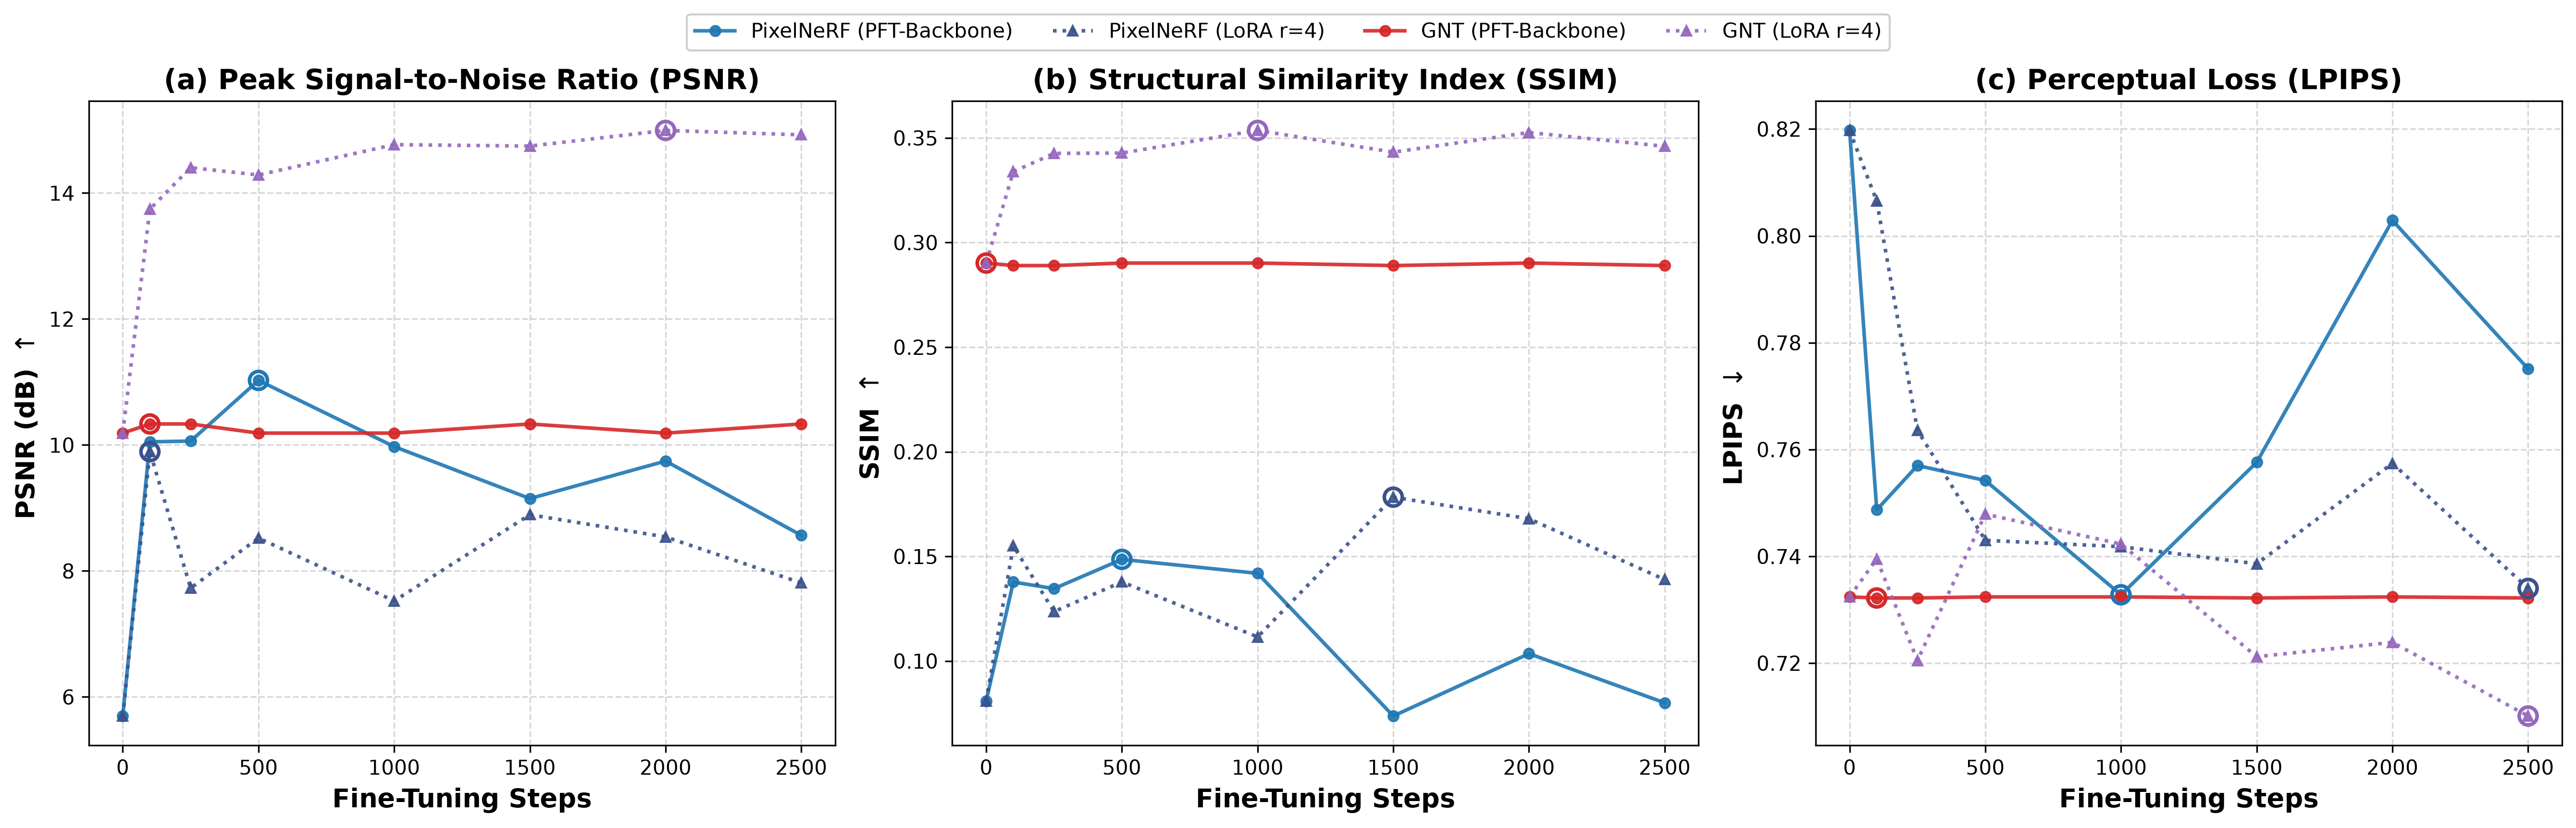
\includegraphics[width=0.88\textwidth]{img/ft_steps_ablation.png}
\vspace{-3pt}
\caption{Ablation of fine-tuning iterations from $0$ (Zero-Shot) to $30,000$ steps on the \textit{fern} scene ($N=3$) for (a) PSNR, (b) SSIM, and (c) LPIPS; circled points mark global optima. PixelNeRF reached its peak between $500$ and $1,000$ steps before degrading due to overfitting ($4.70$ dB under LoRA at $20\text{k}$ steps), whereas GNT with PEFT-LoRA ($r=4$) obtained $>91\%$ of its maximum PSNR gain by $500$ steps ($14.29$ vs.\ $15.59$ dB at $10\text{k}$) and remained stable up to $30\text{k}$ steps.}
\label{fig:ft_steps_ablation}
\end{figure*}

\subsection{Evaluation \& Metrics}
\label{sec:metrics}
All evaluations were executed on the held-out test views (\texttt{llffhold=8}) inside isolated NVIDIA Docker containers using an NVIDIA GeForce GTX 1660 Super GPU (6GB VRAM, CUDA 12.6). Reconstruction quality was measured using PSNR, SSIM \cite{wang2004image}, and VGG-based LPIPS \cite{zhang2018unreasonable, niemeyer2022regnerf}. Computational performance was recorded through total training/adaptation time, rendering throughput in frames per second (FPS) \cite{kulhanek2025nerfbaselinesconsistentreproducibleevaluation}, and peak dynamic VRAM usage allocated by PyTorch during test-view rendering.

\section{Results and Discussion}
\label{sec:results}

This section presents the quantitative, computational, and qualitative results obtained across the LLFF benchmark. Table~\ref{tab:super_results} reports the global averages for reconstruction fidelity, training time, rendering throughput, and dynamic memory allocation across all evaluated regimes.

\begin{table}[!t]
\centering
\caption{Consolidated benchmark results on the LLFF dataset. Values represent global averages across valid test scenes. Training time corresponds to the best 500-step fine-tuning configuration for generalizable models (including test-view evaluation) and 30,000-step convergence for Per-Scene models ($N=10$). VRAM indicates peak dynamic memory allocated during inference.}
\label{tab:super_results}
\scriptsize
\setlength{\tabcolsep}{1.8pt}
\begin{tabular*}{\linewidth}{@{\extracolsep{\fill}}llcccccc@{\extracolsep{0pt}}}
\toprule
Model & Regime 
  & PSNR $\uparrow$ 
  & SSIM $\uparrow$ 
  & LPIPS $\downarrow$ 
  & Time $\downarrow$
  & FPS $\uparrow$ 
  & VRAM $\downarrow$ \\
\midrule
\multirow{2}{*}{PixelNeRF}
 & ZS  & 6.35  & 0.085 & 0.800 & $\sim$22 s   & 0.004 & 1.93 \\
 & FT  & 10.92 & 0.162 & 0.772 & 4 min 36 s   & 0.006 & 1.97 \\
\midrule
\multirow{2}{*}{GNT}
 & ZS  & 10.51 & 0.314 & 0.742 & \textbf{$\sim$9 s}    & 0.014 & 1.94 \\
 & FT  & 15.07 & 0.368 & 0.679 & 4 min 59 s   & 0.015 & 1.93 \\
\midrule
Instant-NGP
 & N=10   & 14.06 & 0.442 & 0.498 & 31 min 51 s  & 0.199 & 1.09 \\
\midrule
Nerfacto
 & N=10   & \textbf{27.11} & \textbf{0.875} & \textbf{0.171} & 8 min 57 s   & 0.388 & 1.43 \\
\midrule
Splatfacto
 & N=10   & 24.80 & 0.830 & 0.210 & 16 min 23 s  & \textbf{200.7} & \textbf{0.10} \\
\bottomrule
\end{tabular*}
\end{table}

\subsection{Visual Fidelity Across Paradigms}
Under $N=10$ input views, per-scene methods that incorporate spatial proposal sampling or explicit 3D primitives achieved the highest visual quality. Nerfacto obtained the best overall metrics at $27.11$ dB PSNR, $0.875$ SSIM, and $0.171$ LPIPS (Table~\ref{tab:super_results}), followed by Splatfacto (3DGS) with $24.80$ dB PSNR, $0.830$ SSIM, and $0.210$ LPIPS. Initializing anisotropic 3D Gaussians from sparse COLMAP point clouds preserved structural boundaries and high-frequency textures across test views. By comparison, Instant-NGP lacked sparse-view depth regularization and overfitted to the training rays, reaching $14.06$ dB PSNR.

For the generalizable architectures, direct Zero-Shot (ZS) inference was affected by domain shift and wide baselines between cameras. PixelNeRF obtained $6.35$ dB PSNR and $0.800$ LPIPS in zero-shot mode, whereas GNT reached $10.51$ dB PSNR and $0.314$ SSIM through its epipolar cross-attention mechanism. After fine-tuning on the target views, GNT improved to $15.07$ dB PSNR (and up to $17.46$ dB on \textit{fortress}), outperforming per-scene Instant-NGP ($14.06$ dB) in less training time ($4\text{ min }59\text{ s}$ vs.\ $31\text{ min }51\text{ s}$). Fine-tuning also raised PixelNeRF by $+4.57$ dB to $10.92$ dB PSNR under backbone adaptation, although its rendered views remained spatially blurred.

\subsection{Comparative Analysis of Fine-Tuning Strategies}
\label{sec:ft_results}

Table~\ref{tab:mixed_model_comparison} and Figure~\ref{fig:ft_efficiency_bars} summarize the multi-seed reconstruction metrics and execution times across the five fine-tuning strategies for PixelNeRF (5 valid scenes) and GNT (6 valid scenes). The results show opposite adaptation requirements between the convolutional and transformer-based architectures.

\begin{table}[!t]
\centering
\caption{Multi-seed evaluation of fine-tuning strategies on PixelNeRF (5 valid scenes) and GNT (6 valid scenes) across seeds $\{42, 123, 999\}$ at $500$ steps. CNN-based PixelNeRF achieved its highest PSNR under encoder adaptation (\textit{PFT-Backbone}), whereas transformer-based GNT performed best under epipolar decoder tuning (\textit{PFT-Decoder}) and low-rank adaptation (\textit{PEFT-LoRA}).}
\label{tab:mixed_model_comparison}
\scriptsize
\setlength{\tabcolsep}{2.5pt}
\begin{tabular*}{\linewidth}{@{\extracolsep{\fill}}llccccc@{\extracolsep{0pt}}}
\toprule
Model & Strategy & $\eta$ & $r$ & PSNR (dB) $\uparrow$ & SSIM $\uparrow$ & LPIPS $\downarrow$ \\
\midrule
\multirow{6}{*}{PixelNeRF}
 & Zero-Shot (ZS)   & N/A        & N/A    & 6.35 $\pm$ 0.05            & 0.085    & 0.800    \\
 & Full-FT          & $10^{-4}$  & N/A    & 9.03 $\pm$ 0.11            & 0.136    & 0.752    \\
 & PFT-Decoder      & $10^{-4}$  & N/A    & 10.58 $\pm$ 0.08           & \textbf{0.205} & 0.773    \\
 & PFT-Backbone     & $10^{-4}$  & N/A    & \textbf{10.92} $\pm$ 0.26  & 0.162    & 0.772    \\
 & BitFit           & $10^{-4}$  & N/A    & 10.79 $\pm$ 0.19           & 0.119    & 0.775    \\
 & PEFT-LoRA        & $10^{-3}$  & 4      & 8.59 $\pm$ 0.10            & 0.175    & \textbf{0.725} \\
\midrule
\multirow{6}{*}{GNT}
 & Zero-Shot (ZS)   & N/A        & N/A    & 10.51 $\pm$ 0.11           & 0.314    & 0.742    \\
 & Full-FT          & $10^{-3}$  & N/A    & 15.06 $\pm$ 0.03           & \textbf{0.369} & 0.681    \\
 & PFT-Decoder      & $10^{-3}$  & N/A    & \textbf{15.07} $\pm$ 0.03  & 0.368    & \textbf{0.679} \\
 & PFT-Backbone     & $10^{-4}$  & N/A    & 10.51 $\pm$ 0.11           & 0.314    & 0.742    \\
 & BitFit           & $10^{-3}$  & N/A    & 13.12 $\pm$ 0.05            & 0.358    & 0.742    \\
 & PEFT-LoRA        & $10^{-3}$  & 4      & 14.57 $\pm$ 0.07           & \textbf{0.369} & 0.706    \\
\bottomrule
\end{tabular*}
\end{table}

\begin{figure}[!t]
\centering
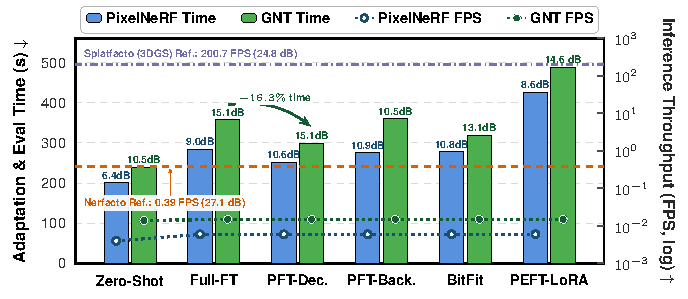
\includegraphics[width=\linewidth]{img/plot_ft_bars.pdf}
\vspace{-4pt}
\caption{Adaptation and evaluation time (bars, left axis, annotated with mean PSNR) and rendering throughput in FPS (markers, right log-axis) across fine-tuning strategies for PixelNeRF and GNT, compared against Nerfacto and Splatfacto (3DGS) reference lines. In GNT, \textit{PFT-Decoder} matched \textit{Full-FT} accuracy ($15.07$ dB) while reducing adaptation time by $16.3\%$ ($298.8\text{ s}$ vs.\ $357.1\text{ s}$). \textit{PEFT-LoRA} ($r=4$) required longer training time ($488.0\text{ s}$) due to adapter projections during backpropagation, but maintained native inference speed ($0.015$ FPS) after in-place weight merging.}
\label{fig:ft_efficiency_bars}
\end{figure}

In PixelNeRF, the highest PSNR was obtained when restricting gradient updates to the ResNet encoder (\textit{PFT-Backbone}, $10.92 \pm 0.26$ dB in $275.7\text{ s}$) or to additive biases (\textit{BitFit}, $10.79 \pm 0.19$ dB in $277.7\text{ s}$), both of which outperformed \textit{Full-FT} ($9.03 \pm 0.11$ dB in $284.8\text{ s}$). Because PixelNeRF projects 2D feature maps onto 3D rays, adjusting the convolutional filters to the target scene illumination improved color consistency, whereas updating all weights simultaneously destabilized the downstream MLP. Table~\ref{tab:mixed_model_comparison} also indicates a difference between pixel-level and perceptual metrics: \textit{PFT-Backbone} maximized PSNR through smooth color averaging, while \textit{PFT-Decoder} reached the highest structural similarity ($0.205$ SSIM in $252.0\text{ s}$) and \textit{PEFT-LoRA} ($r=4$) obtained the lowest perceptual error ($0.725$ LPIPS vs.\ $0.772$ for \textit{PFT-Backbone}) despite a lower PSNR ($8.59$ dB).

In GNT, the best reconstruction quality was achieved under \textit{PFT-Decoder} ($15.07 \pm 0.03$ dB PSNR and $0.679$ LPIPS), matching \textit{Full-FT} ($15.06 \pm 0.03$ dB) while avoiding backpropagation through the ViT encoder and reducing adaptation time from $357.1\text{ s}$ to $298.8\text{ s}$ (a $16.3\%$ reduction, Figure~\ref{fig:ft_efficiency_bars}). Freezing the pre-trained ViT encoder preserved its visual representations and concentrated weight updates within the epipolar cross-attention layers. In contrast, \textit{PFT-Backbone} produced no improvement over Zero-Shot ($10.51 \pm 0.11$ dB in $360.8\text{ s}$), showing that GNT adaptation depends on epipolar ray aggregation rather than shallow 2D patch projections. Parameter-efficient strategies also regularized GNT training: \textit{BitFit} reached $13.12 \pm 0.05$ dB ($+2.61$ dB over ZS in $319.0\text{ s}$) by updating $<0.15\%$ of the weights, and \textit{PEFT-LoRA} ($r=4$) reached $14.57 \pm 0.07$ dB and $0.369$ SSIM. Although evaluating the auxiliary \texttt{LoRALinear} branches during training increased execution time ($488.0\text{ s}$ in GNT and $426.4\text{ s}$ in PixelNeRF), merging $\Delta W = \frac{\alpha}{r}BA$ into $W_0$ before evaluation preserved the baseline rendering speed ($0.015$ and $0.006$ FPS).

\subsection{Computational Efficiency and Pareto Trade-offs}
Figures~\ref{fig:boxplot} and~\ref{fig:radar_chart} present the PSNR distribution across scenes and the five-axis trade-off profile across fidelity and hardware metrics. Generalizable models exhibited low inter-scene variance in Zero-Shot mode, which expanded after fine-tuning as the networks adapted to scene-specific geometry, whereas per-scene models showed wider variance driven by scene texture complexity.

\begin{figure}[!t]
\centering
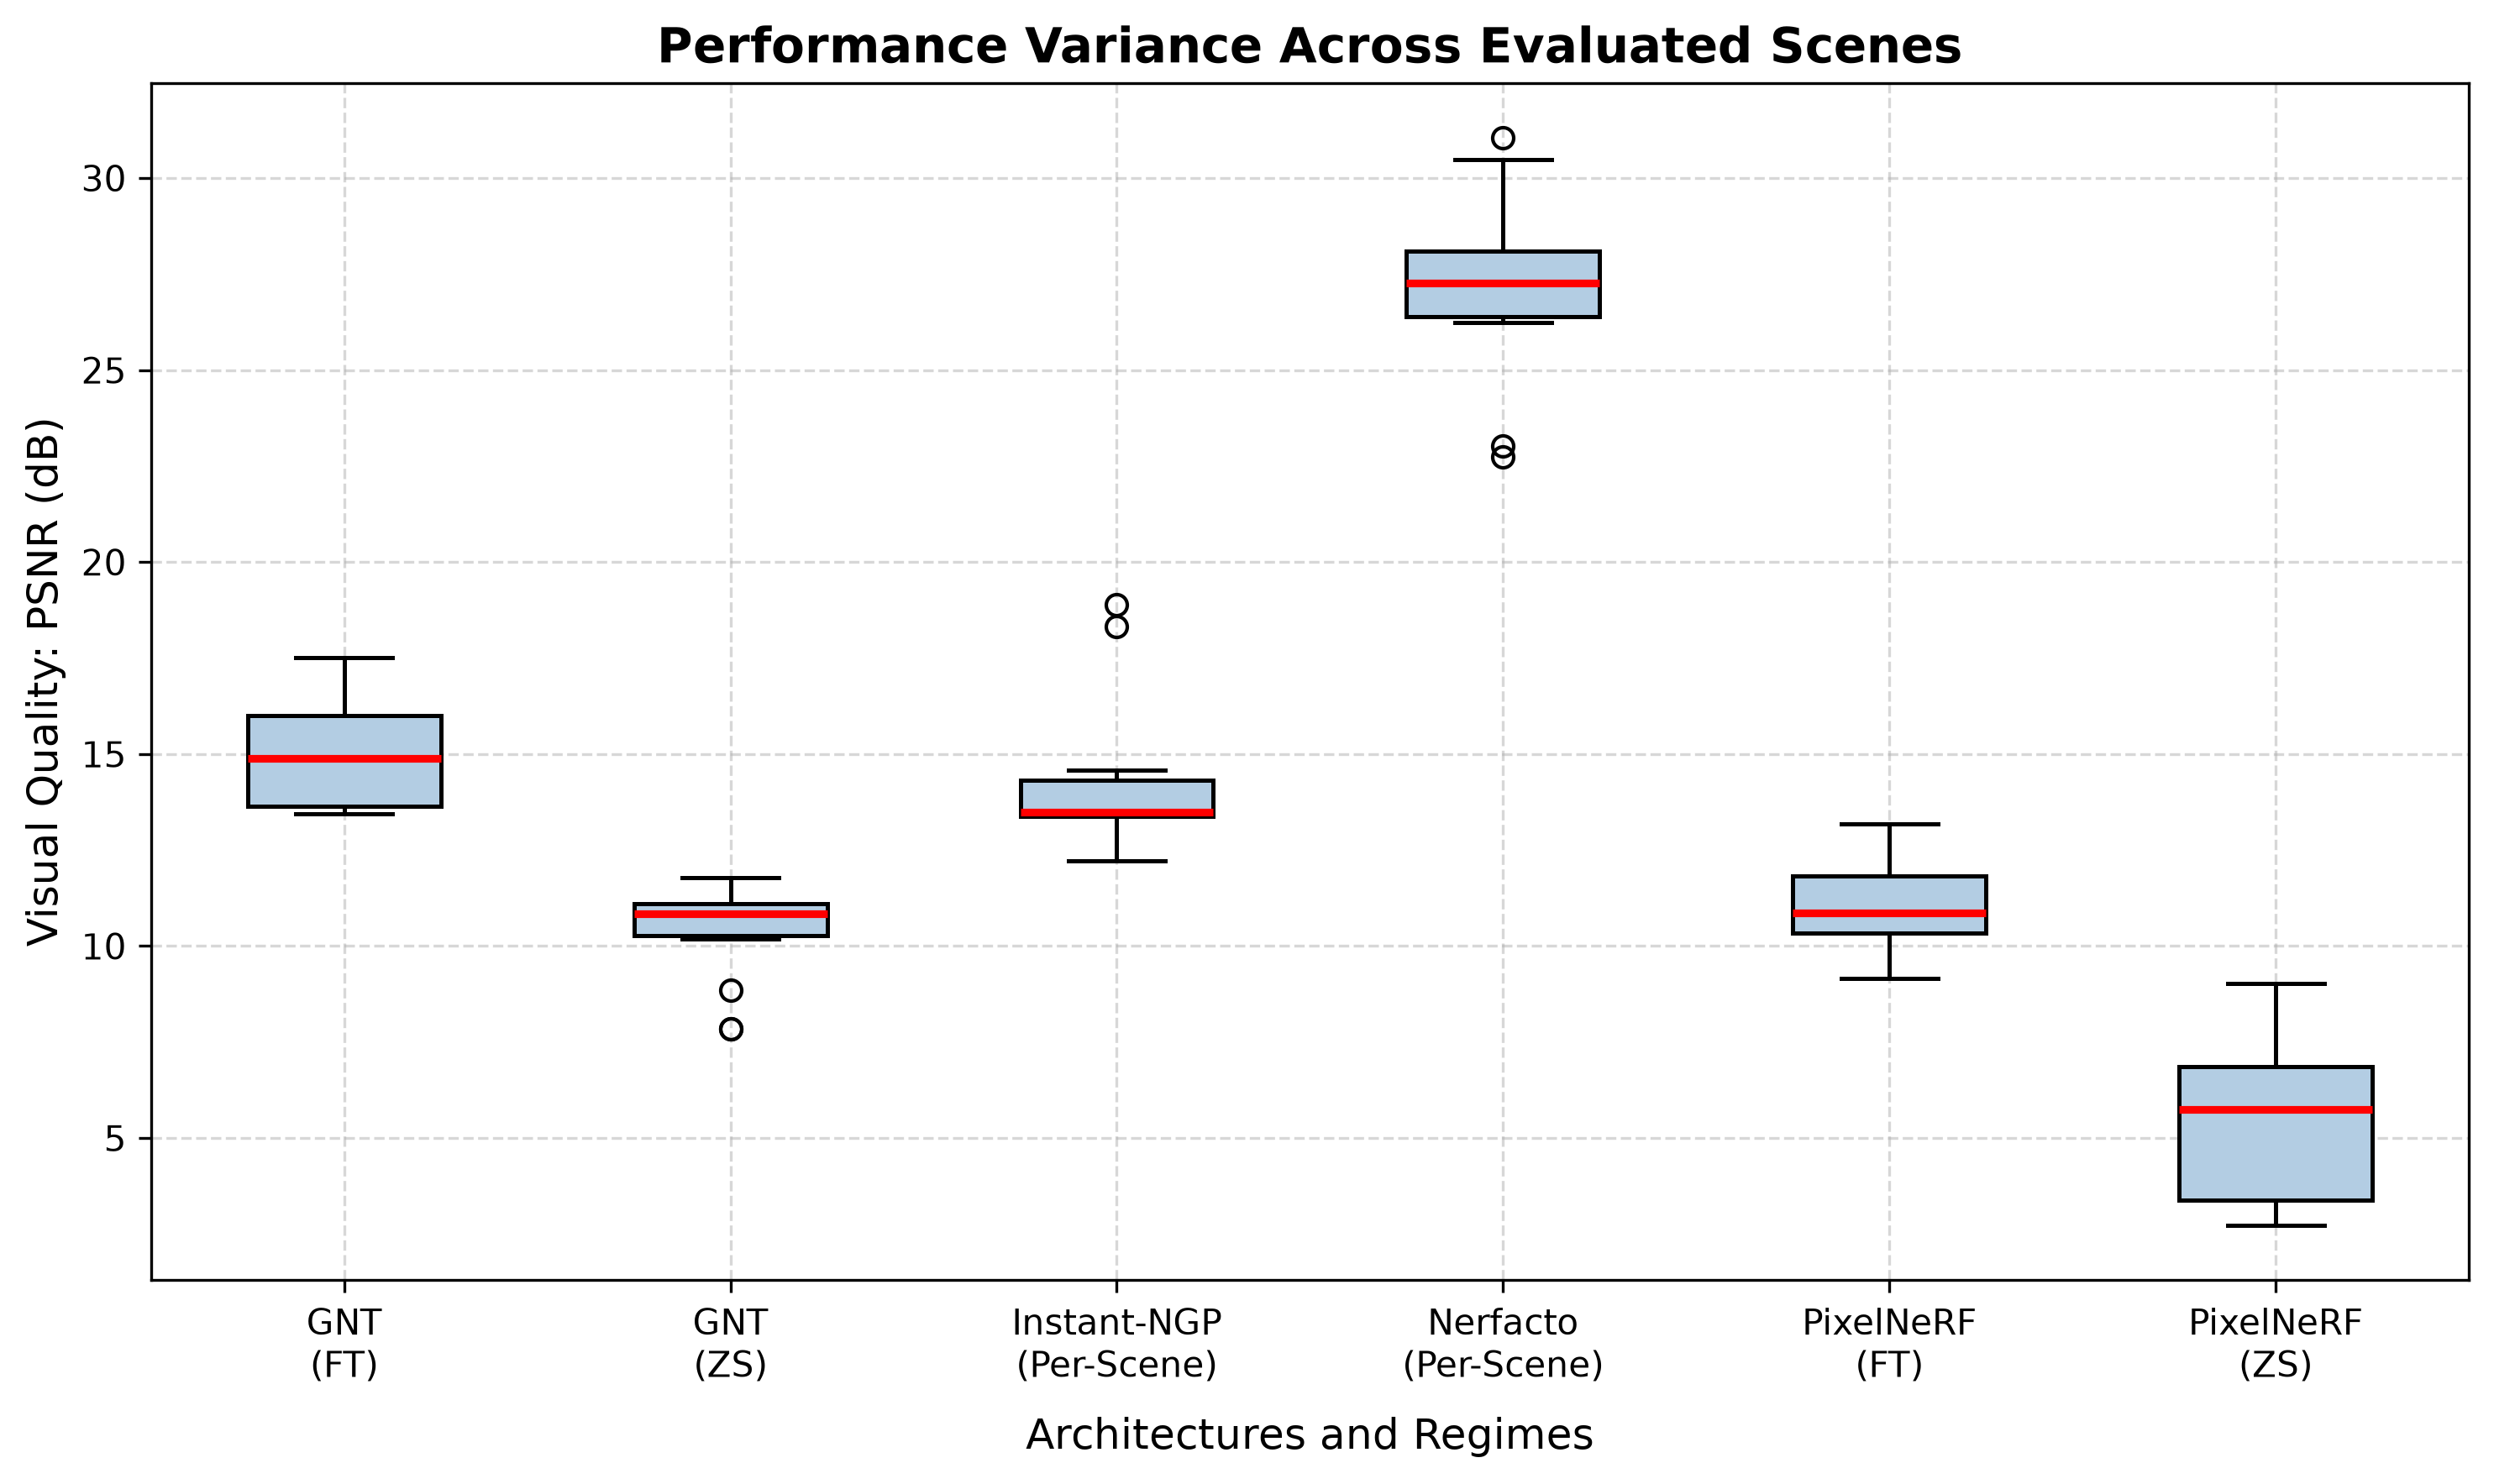
\includegraphics[width=0.84\linewidth]{img/plot_boxplot_fix.png}
\vspace{-3pt}
\caption{PSNR distributions across valid LLFF scenes ($N=10$ for per-scene baselines; optimal FT vs.\ ZS for generalizable models). Red horizontal lines indicate medians and boxes represent interquartile ranges (IQR). Fine-tuned GNT achieved a higher median PSNR than Instant-NGP ($15.07$ vs.\ $14.06$ dB), while Nerfacto reached the highest overall distribution ($27.11$ dB mean).}
\label{fig:boxplot}
\end{figure}

\begin{figure}[!t]
\centering
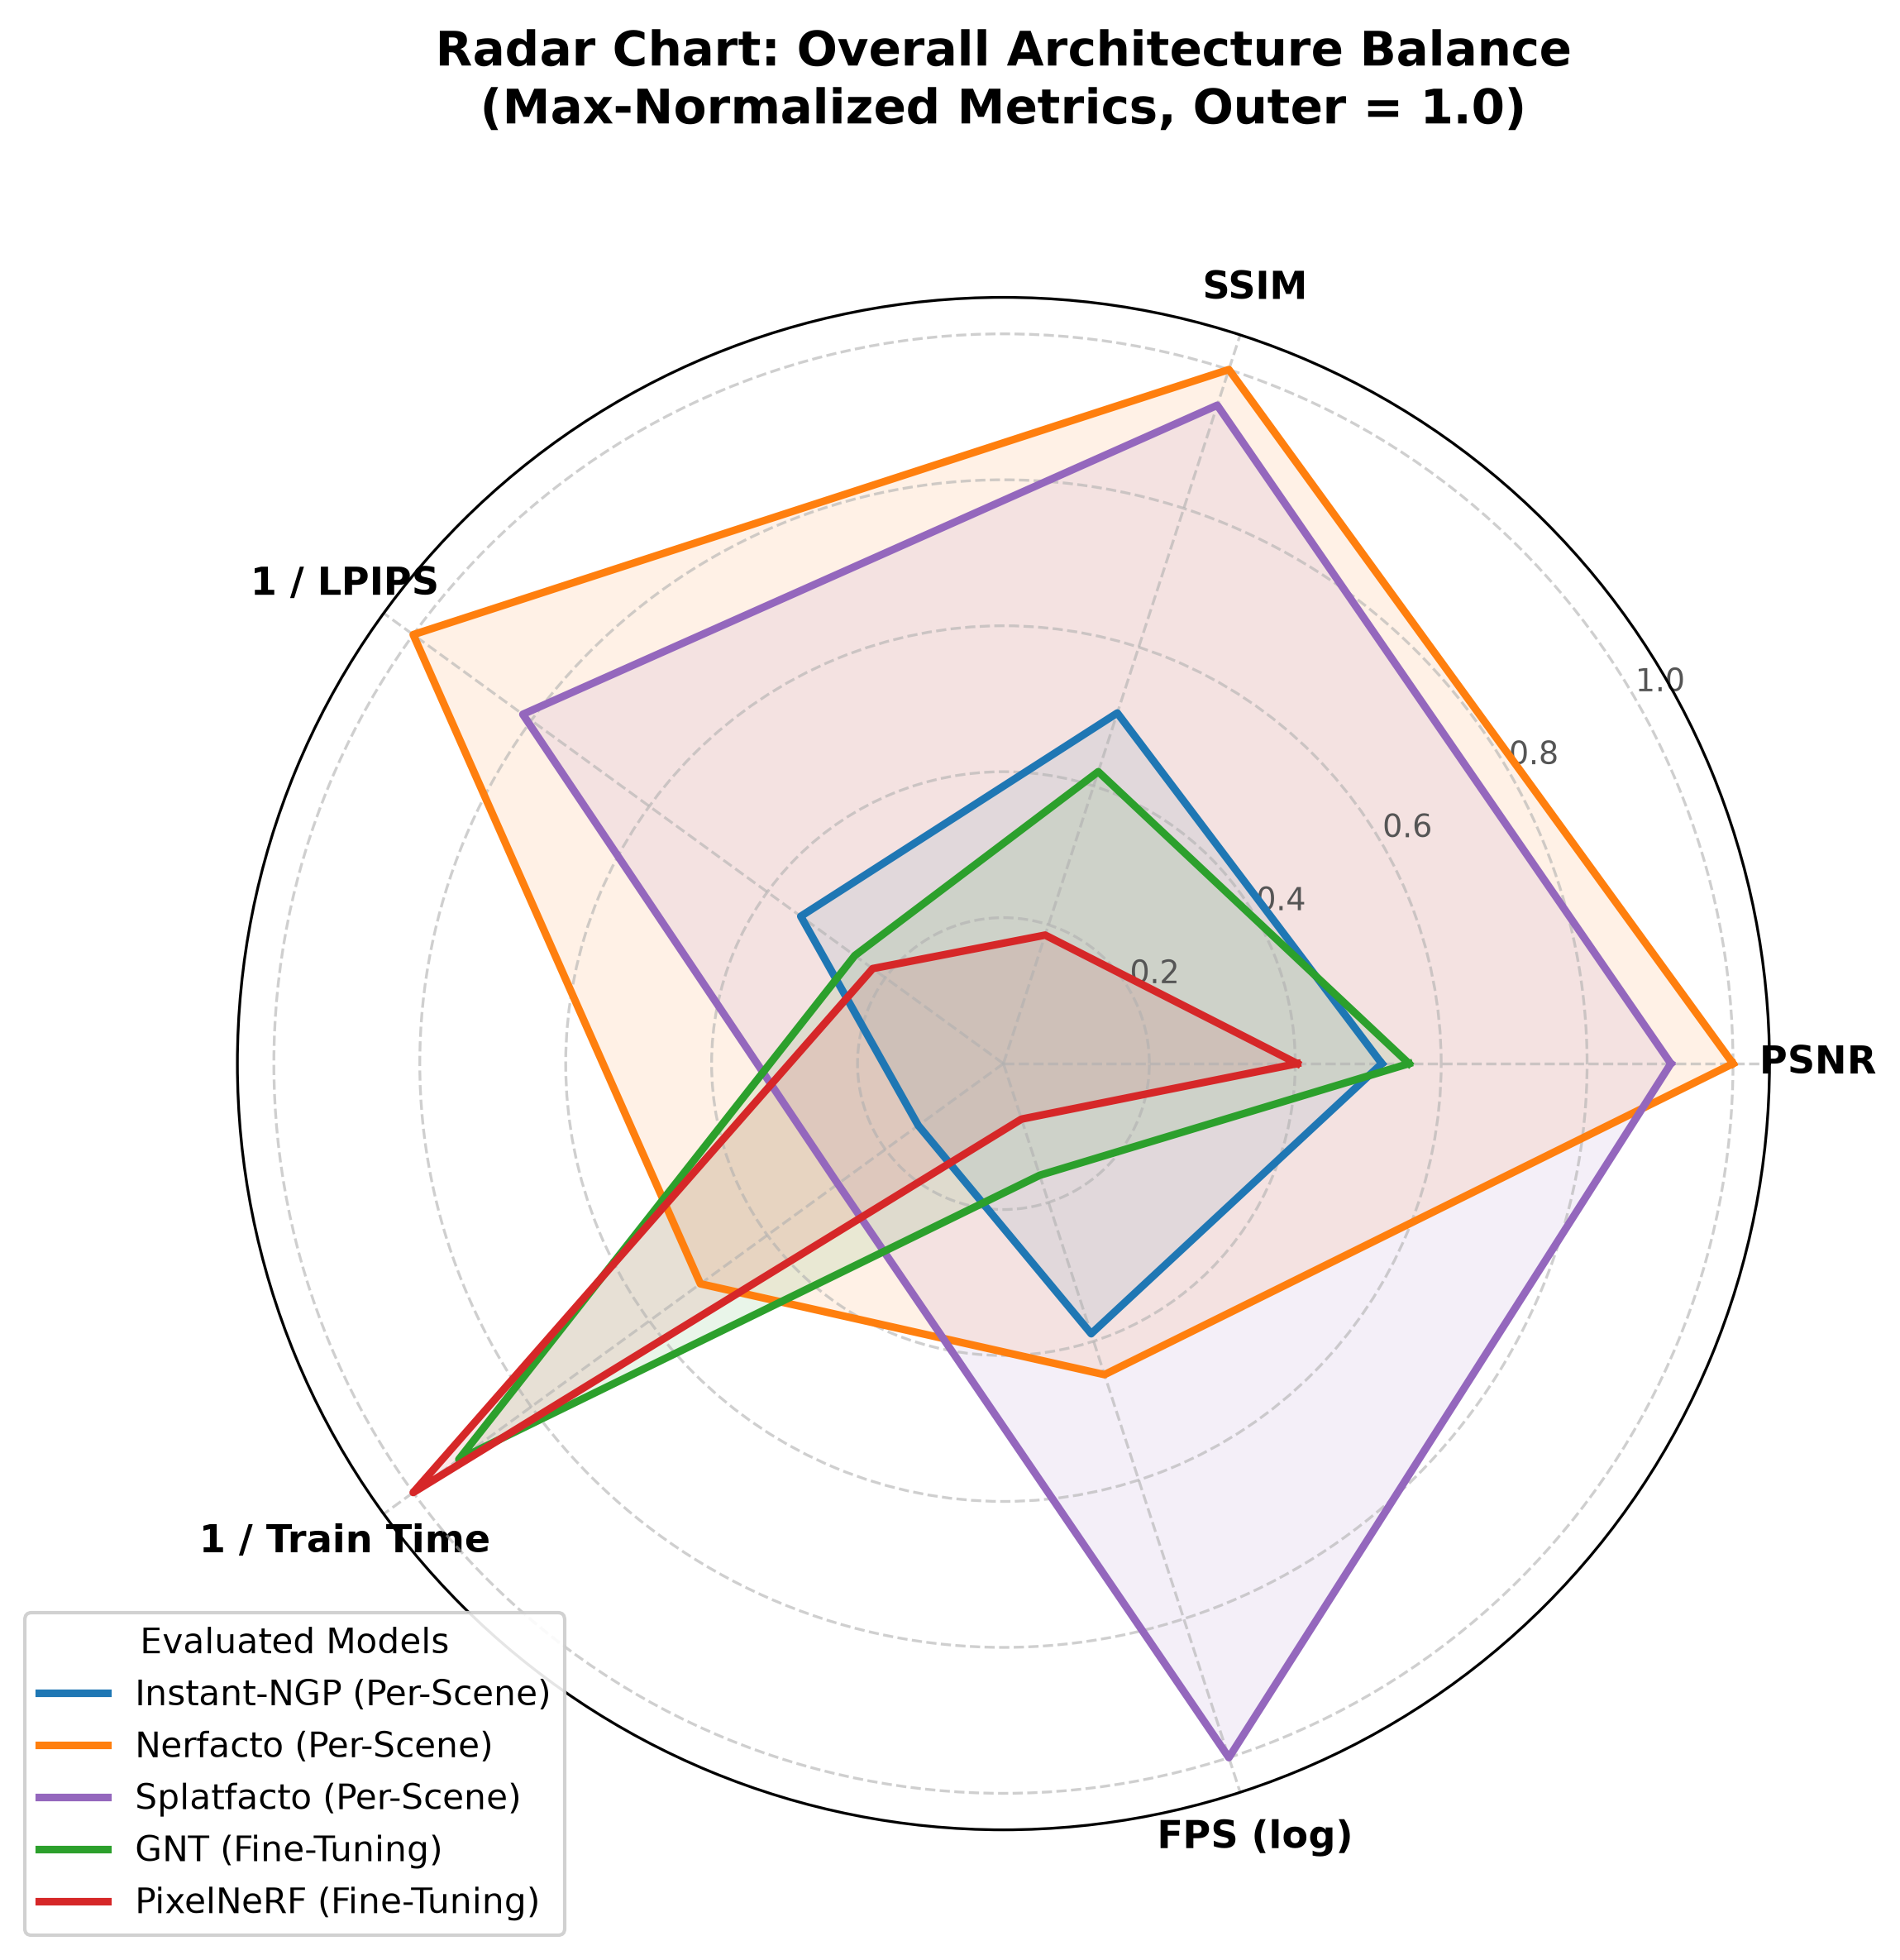
\includegraphics[width=0.74\linewidth]{img/plot_radar_fix.png}
\vspace{-3pt}
\caption{Multi-metric trade-offs under sparse-view conditions ($N=10$). Metrics were max-normalized to $[0,1]$ (outer perimeter = best), using $1/\text{LPIPS}$, $1/\text{Train Time}$, and log-scaled FPS. Splatfacto led in rendering speed ($200.7$ FPS) and Nerfacto led in visual fidelity, whereas fine-tuned GNT required the shortest adaptation time ($\sim 5\text{ min}$) but exhibited low rendering FPS.}
\label{fig:radar_chart}
\end{figure}

Comparing training time against inference throughput highlights the operational trade-off between both families of methods. Generalizable models required only $\sim 9\text{--}22\text{ s}$ for Zero-Shot evaluation or $\sim 4.6\text{--}5.0\text{ min}$ for 500-step fine-tuning, but projecting multi-view features and evaluating epipolar attention along each ray limited rendering throughput to $0.006$ FPS in PixelNeRF and $0.015$ FPS in GNT, with $\sim 1.94$ GB of dynamic VRAM. Per-scene hash-grid models increased inference speed to $0.199$ FPS in Instant-NGP and $0.388$ FPS in Nerfacto. Using explicit tile-based rasterization, Splatfacto (3DGS) reached $200.7$ FPS ($\approx 517\times$ faster than Nerfacto) while consuming $0.10$ GB of dynamic VRAM ($14.3\times$ less than Nerfacto's $1.43$ GB), requiring $16\text{ min }23\text{ s}$ of per-scene optimization. Consequently, PFT- and PEFT-adapted GNT was advantageous under extreme view scarcity ($N=3$) and short adaptation budgets, whereas Splatfacto and Nerfacto were superior when $N \ge 10$ views and longer training times were available.

\subsection{Qualitative Analysis}
Figure~\ref{fig:comparacao_qualitativa} shows novel views rendered across five LLFF scenes (\textit{Fern}, \textit{Flower}, \textit{Fortress}, \textit{Horns}, and \textit{Room}) under $N=10$ input views.

In Column 1, PixelNeRF adapted with \textit{PFT-Backbone} recovered the global color palette and coarse object contours in structured scenes such as \textit{Fortress} and \textit{Room}. However, because its coordinate MLP averages projected features without explicit depth reasoning, scenes with multi-layer occlusions (\textit{Fern} and \textit{Horns}) exhibited heavy spatial smoothing, consistent with its $0.772$ LPIPS score.

Columns 2 to 4 show the visual progression across the GNT fine-tuning strategies as the number of adapted parameters in the decoder increased. In Column 2, \textit{BitFit} ($<0.15\%$ trainable weights) corrected zero-shot color shifts and reduced near-camera floaters, but left fine surface textures blurred. In Column 3, adding rank-$4$ adapters via \textit{PEFT-LoRA} sharpened object boundaries, recovering petal edges in \textit{Flower} and bone contours in \textit{Horns}. In Column 4, updating the full rendering head under \textit{PFT-Decoder} produced the sharpest reconstructions among the generalizable models ($15.07$ dB PSNR and $0.679$ LPIPS), separating overlapping leaves in \textit{Fern} and stone reliefs in \textit{Fortress}.

In Column 5, \textit{Splatfacto} (3DGS) produced the sharpest textures and depth boundaries across all five scenes. The explicit 3D Gaussian primitives reconstructed fine foliage details in \textit{Fern} and \textit{Flower} as well as background structures in \textit{Horns} and \textit{Room} at $200.7$ FPS, showing only localized elongated Gaussian artifacts near image borders where camera overlap was lower.

\begin{figure}[!t]
\centering
\tiny
\setlength{\tabcolsep}{0pt}
\renewcommand{\arraystretch}{0.38}
\begin{tabular}{@{}c@{\hspace{2.2pt}}c@{\hspace{1.1pt}}c@{\hspace{1.1pt}}c@{\hspace{1.1pt}}c@{\hspace{1.1pt}}c@{}}
& \shortstack{\textbf{PixelNeRF}\\\tiny (Backbone)} & \shortstack{\textbf{GNT}\\\tiny (BitFit)} & \shortstack{\textbf{GNT}\\\tiny (LoRA)} & \shortstack{\textbf{GNT}\\\tiny (Decoder)} & \shortstack{\textbf{Splatfacto}\\\tiny (3DGS)} \\[1.8pt]
\raisebox{13pt}{\textbf{Fern}} &

\includegraphics[width=0.174\linewidth]{img/grid5x5/fern_pixelnerf_ft.png} &
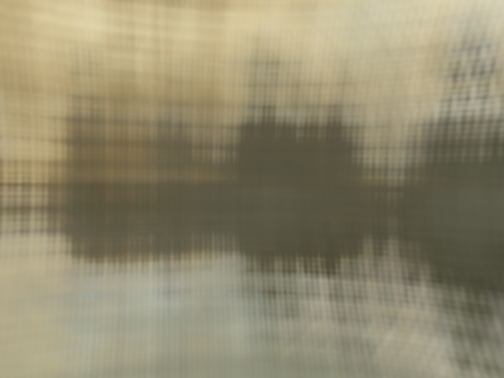
\includegraphics[width=0.174\linewidth]{img/grid5x5/fern_gnt_bitfit.png} &
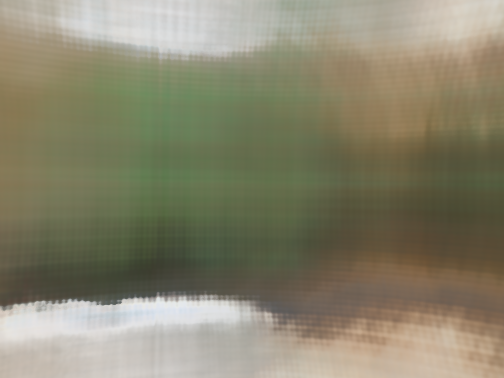
\includegraphics[width=0.174\linewidth]{img/grid5x5/fern_gnt_lora.png} &
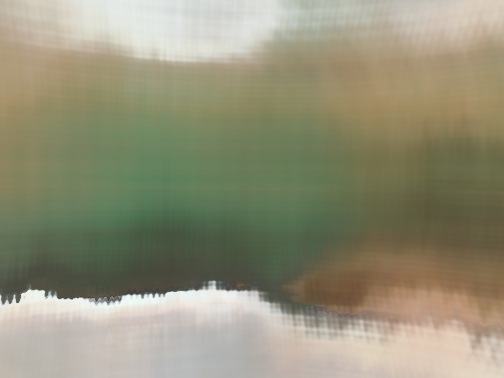
\includegraphics[width=0.174\linewidth]{img/grid5x5/fern_gnt_ft.png} &
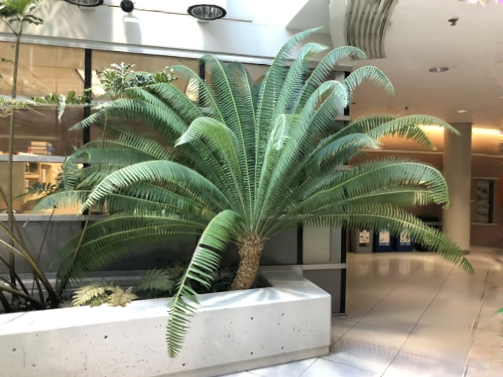
\includegraphics[width=0.174\linewidth]{img/grid5x5/fern_splatfacto.png} \\[1.0pt]
\raisebox{13pt}{\textbf{Flower}} &

\includegraphics[width=0.174\linewidth]{img/grid5x5/flower_pixelnerf_ft.png} &
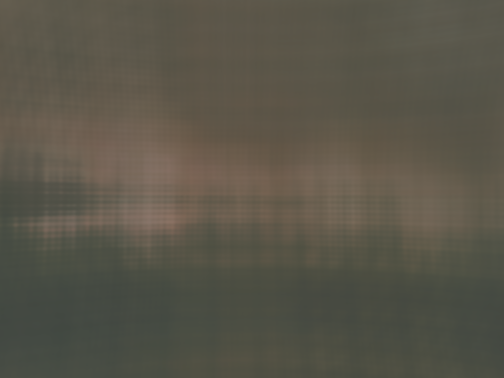
\includegraphics[width=0.174\linewidth]{img/grid5x5/flower_gnt_bitfit.png} &
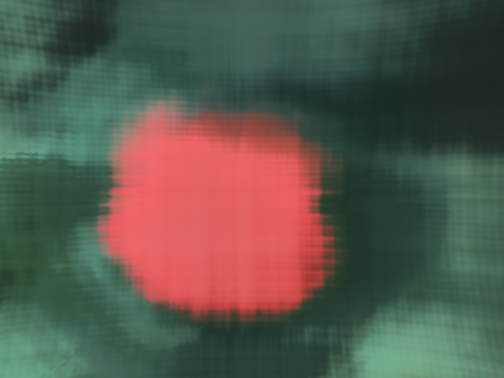
\includegraphics[width=0.174\linewidth]{img/grid5x5/flower_gnt_lora.png} &
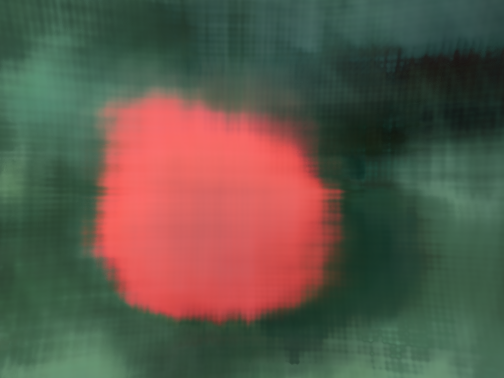
\includegraphics[width=0.174\linewidth]{img/grid5x5/flower_gnt_ft.png} &
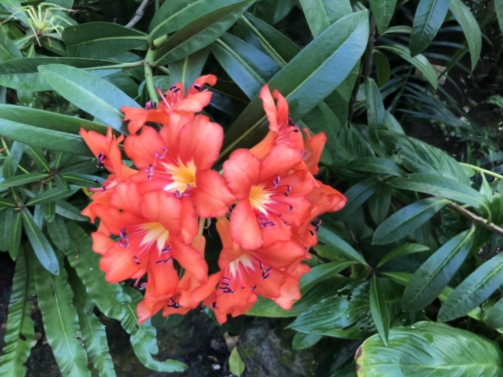
\includegraphics[width=0.174\linewidth]{img/grid5x5/flower_splatfacto.png} \\[1.0pt]
\raisebox{13pt}{\textbf{Fortress}} &

\includegraphics[width=0.174\linewidth]{img/grid5x5/fortress_pixelnerf_ft.png} &
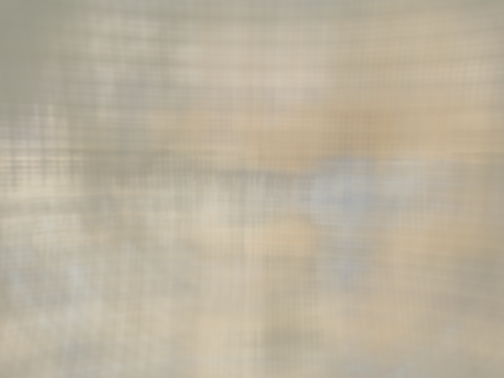
\includegraphics[width=0.174\linewidth]{img/grid5x5/fortress_gnt_bitfit.png} &
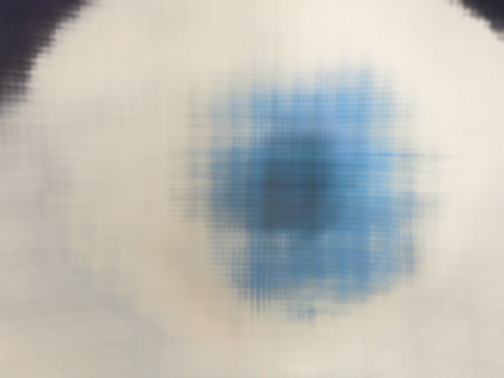
\includegraphics[width=0.174\linewidth]{img/grid5x5/fortress_gnt_lora.png} &
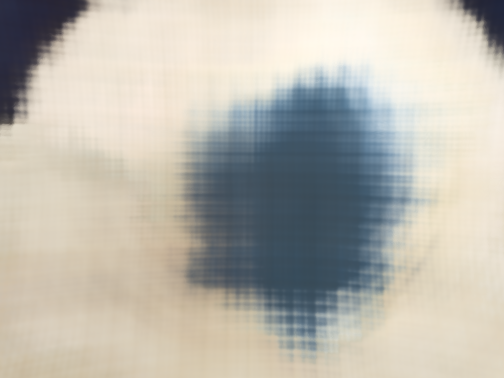
\includegraphics[width=0.174\linewidth]{img/grid5x5/fortress_gnt_ft.png} &
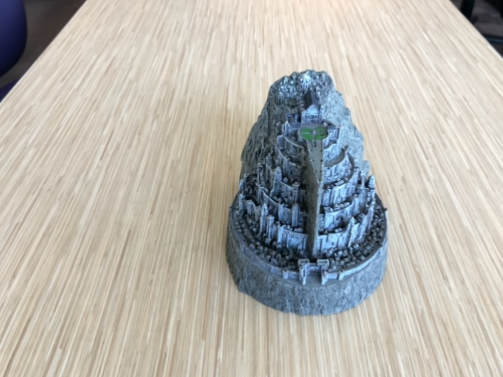
\includegraphics[width=0.174\linewidth]{img/grid5x5/fortress_splatfacto.png} \\[1.0pt]
\raisebox{13pt}{\textbf{Horns}} &

\includegraphics[width=0.174\linewidth]{img/grid5x5/horns_pixelnerf_ft.png} &

\includegraphics[width=0.174\linewidth]{img/grid5x5/horns_gnt_bitfit.png} &
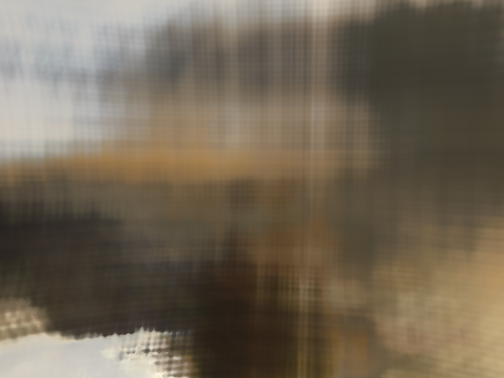
\includegraphics[width=0.174\linewidth]{img/grid5x5/horns_gnt_lora.png} &
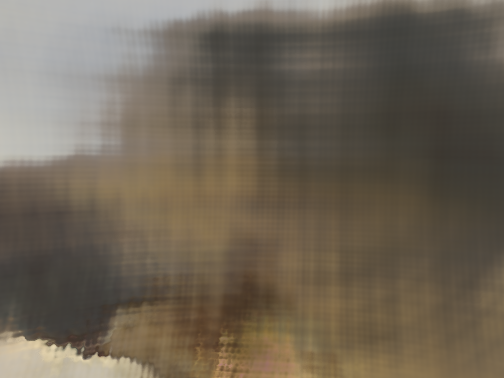
\includegraphics[width=0.174\linewidth]{img/grid5x5/horns_gnt_ft.png} &
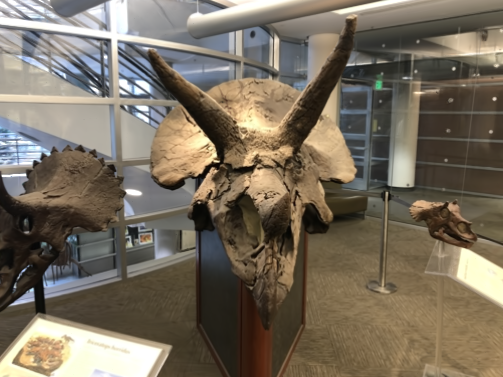
\includegraphics[width=0.174\linewidth]{img/grid5x5/horns_splatfacto.png} \\[1.0pt]
\raisebox{13pt}{\textbf{Room}} &

\includegraphics[width=0.174\linewidth]{img/grid5x5/room_pixelnerf_ft.png} &
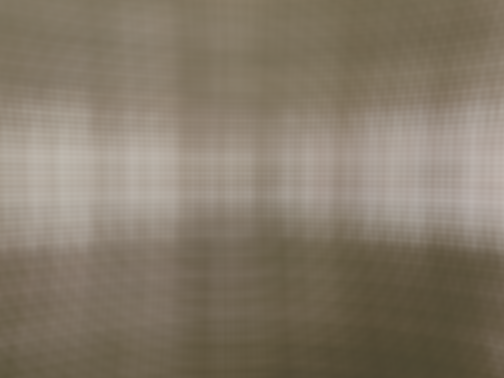
\includegraphics[width=0.174\linewidth]{img/grid5x5/room_gnt_bitfit.png} &
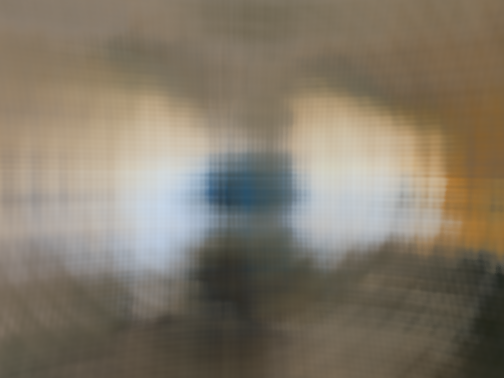
\includegraphics[width=0.174\linewidth]{img/grid5x5/room_gnt_lora.png} &
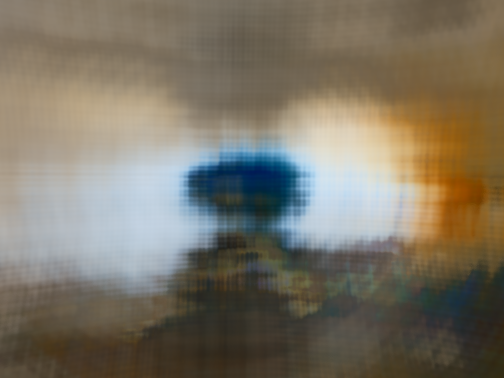
\includegraphics[width=0.174\linewidth]{img/grid5x5/room_gnt_ft.png} &
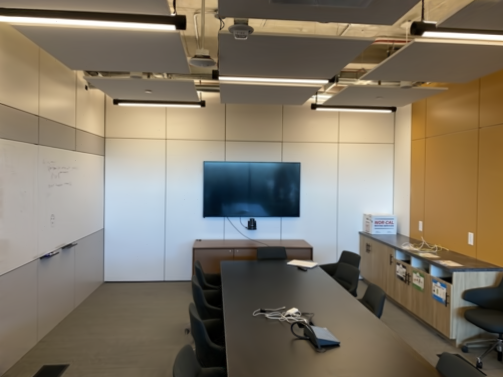
\includegraphics[width=0.174\linewidth]{img/grid5x5/room_splatfacto.png} \\
\end{tabular}
\vspace{-4pt}
\caption{Qualitative comparison across five LLFF scenes under $N=10$ input views. From left to right: PixelNeRF adapted with PFT-Backbone (Col.\ 1), GNT adapted with BitFit (Col.\ 2), PEFT-LoRA ($r=4$, Col.\ 3), and PFT-Decoder (Col.\ 4), and per-scene Splatfacto / 3DGS (Col.\ 5). Increasing the adapted parameter capacity in the GNT decoder progressively sharpened object contours, while Splatfacto preserved the finest high-frequency details at $>200$ FPS.}
\label{fig:comparacao_qualitativa}
\end{figure}

\section{Conclusion}

This work presented a reproducible benchmarking methodology to evaluate reconstruction fidelity, adaptation stability, and computational efficiency across generalizable and per-scene neural rendering architectures under sparse-view conditions. In the experimental evaluation, per-scene models achieved the best visual quality and rendering speed under $N=10$ views: Nerfacto reached $27.11$ dB PSNR and $0.171$ LPIPS, while Splatfacto (3DGS) rendered novel views at $200.7$ FPS using $0.10$ GB of dynamic VRAM. Under three input views ($N=3$), modular fine-tuning of pre-trained priors prevented representational collapse: adapting GNT via \textit{PFT-Decoder} ($15.07$ dB) or \textit{PEFT-LoRA} ($14.57$ dB) reduced adaptation time by $16.3\%$ compared to full fine-tuning and outperformed Instant-NGP ($14.06$ dB), although limited by volumetric ray-marching throughput ($\le 0.015$ FPS).

Future work will extend this evaluation protocol to unbounded $360^\circ$ scenes and investigate depth-regularized sparse-view 3D Gaussian Splatting methods \cite{seo2026improvingsparseview3dgsgeneralization, song2025d2gsdepthanddensityguidedgaussian} alongside feed-forward Gaussian architectures.

\section*{Acknowledgment}
The authors gratefully acknowledge the financial support of the National Council for Scientific and Technological Development - CNPq (Grants \#305386/2024-7, \#302833/2025-0, \#307318/2022-2 and \#404571/2025-5), the State of Minas Gerais Research Foundation - FAPEMIG (Grant \#APQ-00727-24 and \#APD-01428-25) and the State of São Paulo Research Foundation - FAPESP (Grant \#2022/03020-1).

% references section

\bibliographystyle{IEEEtran}
\bibliography{example}
\end{document}
